\documentclass[10pt,a4paper]{article}

\usepackage[english]{babel}
\usepackage[utf8]{inputenc}
\usepackage[T1]{fontenc}
\usepackage[a4paper, margin=1.3cm]{geometry}
\setlength{\columnsep}{0.4cm}
\setlength{\parskip}{0.3ex}
\setlength{\parindent}{0pt}

% Reduce spacing around section headings
\usepackage{titlesec}
\titlespacing*{\section}{0pt}{0.8ex}{0.4ex}
\titlespacing*{\subsection}{0pt}{0.6ex}{0.2ex}

% Reduce spacing in figures and tables
\setlength{\abovecaptionskip}{2pt}
\setlength{\belowcaptionskip}{2pt}
\usepackage{amsmath,amsfonts,amssymb}
\usepackage[colorlinks]{hyperref}
\usepackage{multicol}
\usepackage{graphicx}
\usepackage{float}
\usepackage{booktabs}

\usepackage[round]{natbib}
\bibliographystyle{abbrvnat}

\usepackage{fancyhdr}
\pagestyle{fancy}
\fancyhead[L]{02460-2026 Mini-project 1}
\fancyhead[R]{s250201, s271828 \& s314159}

% For including code
% From https://www.overleaf.com/learn/latex/Code_listing
\usepackage{listings}
\usepackage{xcolor}

\definecolor{codegreen}{rgb}{0,0.6,0}
\definecolor{codegray}{rgb}{0.5,0.5,0.5}
\definecolor{codepurple}{rgb}{0.58,0,0.82}
\definecolor{backcolour}{rgb}{0.95,0.95,0.92}

\lstdefinestyle{mystyle}{
    backgroundcolor=\color{backcolour},   
    commentstyle=\color{codegreen},
    keywordstyle=\color{magenta},
    numberstyle=\tiny\color{codegray},
    stringstyle=\color{codepurple},
    basicstyle=\ttfamily\footnotesize,
    breakatwhitespace=false,         
    breaklines=true,                 
    captionpos=b,                    
    keepspaces=true,                 
    numbers=left,                    
    numbersep=5pt,                  
    showspaces=false,                
    showstringspaces=false,
    showtabs=false,                  
    tabsize=2,
    upquote=true
}

\lstset{language=Python, style=mystyle}

\usepackage{lipsum}

\begin{document}

%%% Main text part %%%

\section*{Mini-project 1 in Advanced Machine Learning (02460)}
by Nikolaos Iliakis (s250201), Konstantinos Bantos (s253777) \& Eve (s314159) on 05 March 2026

\begin{multicols}{2}
    \subsection*{Part A: Priors for variational autoencoders (VAEs)}
    We consider three different priors for \textbf{VAEs}; a \textbf{standard Gaussian}, a \textbf{mixture of Gaussians} (MoG) and a \textbf{Flow-based} prior. Both the encoder and decoder consist of three linear layers, with ReLU functions after the first two. The encoder receives a 784-dimensional input and outputs a 40-dimensional vector. The decoder maps from the 20-dimensional latent space to a 784-dimensional vector.

    
    The Gaussian prior is fixed and produces a circular distribution\cite{tomczak2024}. As a result, the aggregate posterior is forced to move to fit the prior (Figure \ref{fig:plots}), leading to a non-optimal match between the two. The digit clusters also overlap severely. The MoG prior achieves a more optimal match; more clusters are formed in the latent space, which comes in line with the clusters produced by the aggregate posterior. Finally, the Flow-based prior provides the best match. It is very flexible \cite{tomczak2024}, and thus it is closer to the structure of the aggregate posterior. The clusters overlap much less in this case(Figure \ref{fig:plots}).
    \begin{figure}[H]
        \centering
        \includegraphics[width=2.5cm,height=2.5cm]{gaussian_prior.png}
        \includegraphics[width=2.5cm,height=2.5cm]{mog_prior.png}
        \includegraphics[width=2.5cm,height=2.5cm]{flow_prior.png}
        \includegraphics[width=2.5cm,height=2.5cm]{gaussian_posterior.png}
        \includegraphics[width=2.5cm,height=2.5cm]{mog_posterior.png}
        \includegraphics[width=2.5cm,height=2.5cm]{flow_posterior.png}
        \caption{Prior (top) vs aggregate posterior (bottom) for the three VAEs: Gaussian, MoG, Flow (from left to right)}
        \label{fig:plots}
    \end{figure}
    \begin{table}[H]
        \caption{Mean and Standard Deviation (Std) for test set ELBO across the three priors}
        \begin{center}
            \begin{tabular}{lcc}
                \toprule
                Priors & Mean & Std \\
                \midrule
                Standard Gaussian & -81.6675 &  0.5670 \\
                MoG & -80.1554 & 0.1622 \\
                Flow-based & -72.7806 & 0.1167 \\
                \bottomrule
             \end{tabular}                
        \end{center}
    \end{table}
  The test set log-likelihood was approximated by the ELBO. After 5 training runs, the Gaussian prior has the poorest performance, with a low ELBO mean of -81.67 and a Standard Deviation (std) of 0.57 (Table 1). This proves a difficulty of fitting the data and a very high variance, thus training instability. MoG prior achieves a higher mean and a lower std. The Flow-based prior outperforms the previous priors, providing the highest mean and lowest std. As a result, the more expressive and flexible the model, the tighter the ELBO.


    \subsection*{Part B: Sampling quality of generative models}
    We investigate sampling quality of \textbf{Denoising Diffusion Probabilistic Models} (DDPM) trained on MNIST: (1) UNet in pixel space, and (2) latent diffusion with a $\beta$-VAE encoder. The UNet has channels [32,64,128,256] with skip connections; the latent DDPM uses a 3-layer FC network (256 hidden units) on 32-dim latents. We evaluate quality using FID scores.
    \begin{figure}[H]
        \centering
        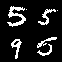
\includegraphics[width=2.5cm,height=2.5cm]{report_images/flow_samples.png}
        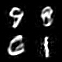
\includegraphics[width=2.5cm,height=2.5cm]{report_images/ddpm_latent_beta1e-3_samples_1.png}
        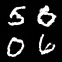
\includegraphics[width=2.5cm,height=2.5cm]{report_images/ddpm_unet_samples_1.png}
        \caption{Generated samples: flow prior VAE (left), latent DDPM with $\beta=10^{-3}$ (center), and pixel-space UNet DDPM (right).}
        \label{fig:ddpm_samples}
    \end{figure}
    \begin{table}[H]
        \caption{FID scores: Part A (flow prior VAE) and Part B (DDPM models).}
        \begin{center}
            \begin{tabular}{lcc}
                \toprule
                Model & FID & Sampling (samples/sec) \\
                \midrule
                Flow prior VAE (Part A) & 6.90 & 20638 \\
                Latent DDPM ($\beta=10^{-6}$) & 5.46 & 2468 \\
                Latent DDPM ($\beta=10^{-3}$) & 4.67 & 2431 \\
                Latent DDPM ($\beta=10^{-2}$) & 5.02 & 2730 \\
                UNet DDPM (pixel space) & 10.17 & 2.33 \\
                \bottomrule
             \end{tabular}
        \end{center}
    \end{table}
    Latent DDPM achieves superior FID ($4.67$ at $\beta=10^{-3}$) vs. flow VAE ($6.90$) and UNet ($10.17$). The $\beta$ parameter controls the trade-off: $\beta=10^{-6}$ (FID$=5.46$) enforces prior alignment; $\beta=10^{-2}$ (FID$=5.02$) favors reconstruction. Sampling speed varies dramatically: VAE (20k/s) $\gg$ latent DDPM ($\sim$2.5k/s) $\gg$ UNet (2.3/s), showing latent diffusion balances quality and efficiency.
    \begin{figure}[H]
        \centering
        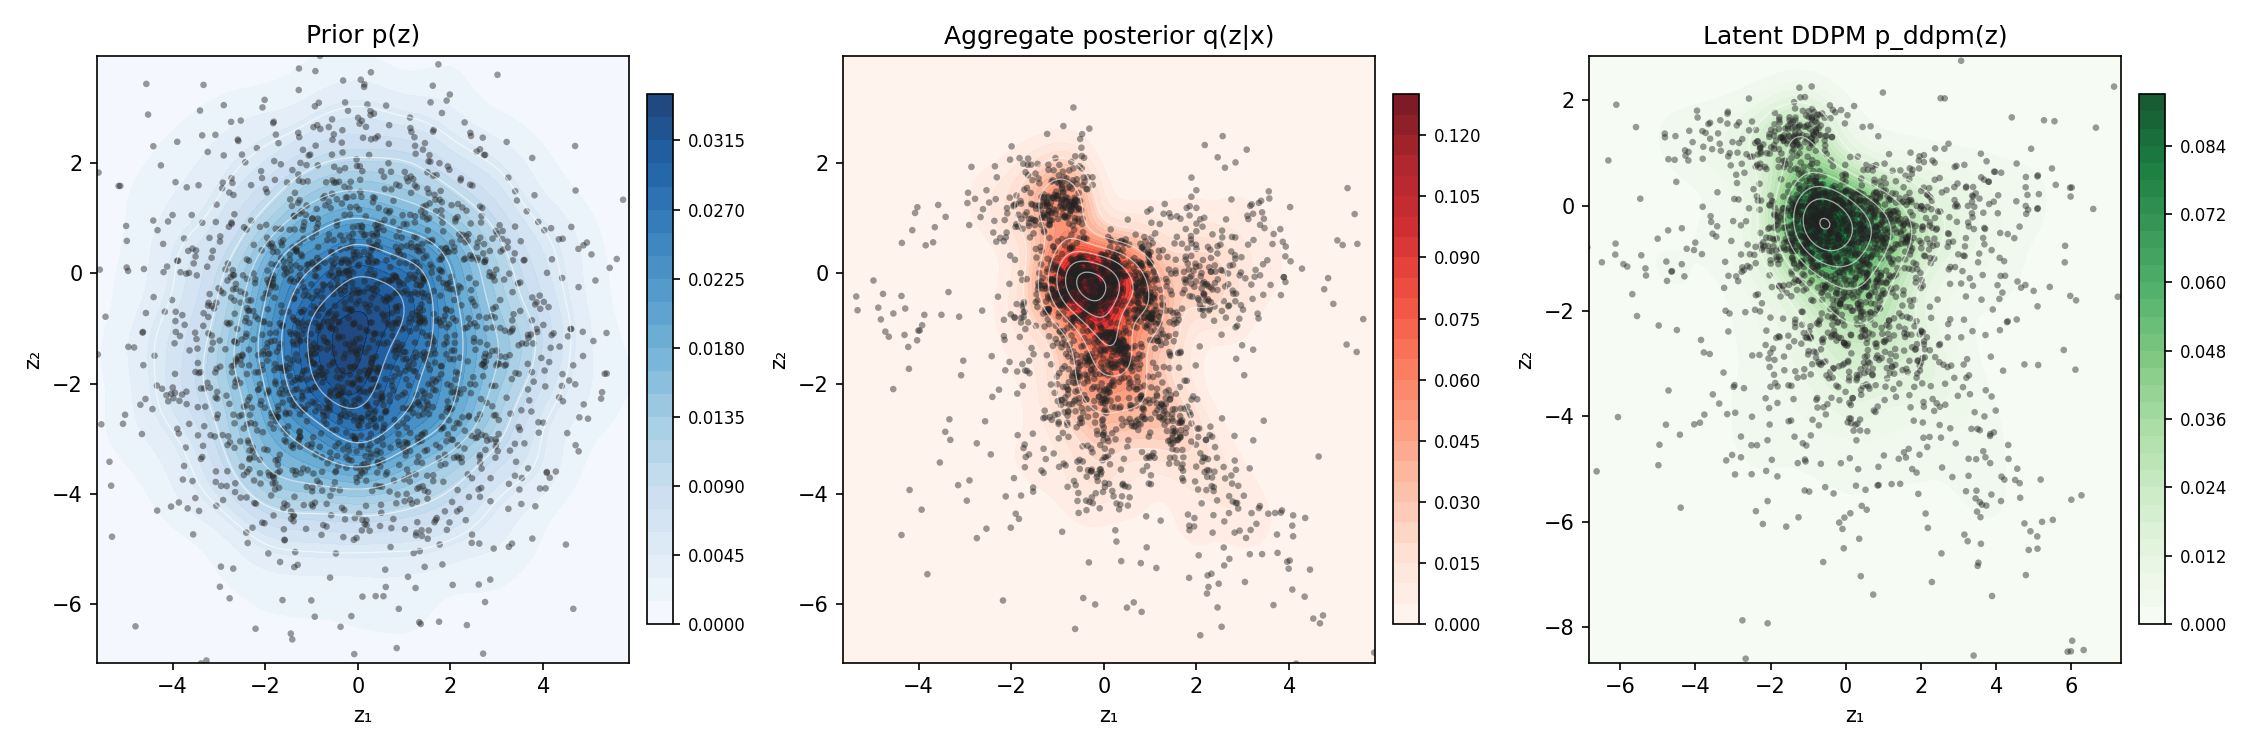
\includegraphics[width=7cm,height=2.5cm]{report_images/latent_comparison.png}
        \caption{$\beta$-VAE prior (left), aggregate posterior (center), and latent DDPM distribution (right). The DDPM learns to match the complex aggregate posterior better than the simple Gaussian prior.}
        \label{fig:prior_comparison}
    \end{figure}
\end{multicols}

\newpage

%%% Code snippet part %%%

\section*{Code snippets}

\subsection*{VAE ELBO Evaluation with Non-Gaussian Priors}
The ELBO for a VAE with an arbitrary prior is computed as: $\text{ELBO} = \mathbb{E}_q[\log p(x|z)] - \beta \cdot \text{KL}(q(z|x) \| p(z))$. For non-Gaussian priors (MoG, Flow), we use Monte Carlo estimation:
\begin{lstlisting}
def elbo(self, x):
    q = self.encoder(x)
    z = q.rsample()
    rec = self.decoder(z).log_prob(x)
    
    if isinstance(self.prior, GaussianPrior):
        kl = td.kl_divergence(q, self.prior())  # closed-form
    else:
        # MC estimate for MoG and Flow
        log_q = q.log_prob(z)
        log_p = self.prior.log_prob(z)
        kl = log_q - log_p  # shape: (batch,)
    
    return torch.mean(rec - self.beta * kl)
\end{lstlisting}

\subsection*{Normalizing Flow Prior}
The flow prior transforms base noise through learned affine coupling layers. Density evaluation uses the inverse flow; sampling uses the forward pass:
\begin{lstlisting}
def log_prob(self, z):
    z0, log_det_J = self.forward(z)  # inverse
    return self.base().log_prob(z0) + log_det_J

def sample(self, n):
    z = self.base().sample(torch.Size([n]))
    for layer in self.layers:  # forward pass
        z, _ = layer.forward(z)
    return z
\end{lstlisting}

\subsection*{DDPM Negative ELBO}
The DDPM loss trains a network to predict noise at random timesteps:
\begin{lstlisting}
def negative_elbo(self, x):
    noise = torch.randn_like(x)
    t = torch.randint(0, self.T, (x.shape[0],))
    noisy = torch.sqrt(self.alpha_cumprod[t]) * x + \
            torch.sqrt(1 - self.alpha_cumprod[t]) * noise
    t_input = (t.float() / self.T).unsqueeze(1)
    pred_noise = self.network(noisy, t_input)
    return ((noise - pred_noise)**2).mean(dim=1)
\end{lstlisting}

\subsection*{Latent DDPM: Training and Sampling}
For latent diffusion, we freeze the VAE encoder/decoder and train DDPM on latent vectors:
\begin{lstlisting}
def negative_elbo(self, x):
    z = self.encode(x)
    return self.ddpm.negative_elbo(z)

def sample(self, n_samples):
    z_samples = self.ddpm.sample((n_samples, self.latent_dim))
    x_samples = self.decode(z_samples)
    return x_samples
\end{lstlisting}

\newpage


%%% AI declaration %%%

\section*{Declaration of use of generative AI}

This declaration \textbf{must} be filled out and included as the 3rd page of the document. The questions apply to all parts of the work, including research, project writing, and coding.
\begin{itemize}
\item I/we have used generative AI tools: [yes]
\end{itemize}
If you answered \emph{yes}, please complete the following sections. List the generative AI tools you have used:
\begin{itemize}
\item GitHub Copilot
\end{itemize}
Describe how the tools were used:
\begin{description}
\item[What did you use the tool(s) for?] Helper scripts for data loading and FID computation CLI tools. Report writing and refinement for clarity and grammar in parts of the manuscript.
\item[At what stage(s) of the process did you use the tool(s)?] During implementation of utility scripts (early stage) and during final report writing and editing (late stage).
\item[How did you use or incorporate the generated output?] Generated code templates were reviewed and integrated into the project structure. Suggested text improvements were evaluated and selectively incorporated into the final report.
\end{description}

\newpage

%%% Bibliography %%%

\bibliography{template}

\end{document}
